\documentclass[11pt]{beamer}
\usetheme{Madrid}
\usepackage[utf8]{inputenc}
\usepackage{amsmath, amssymb, amsfonts, amsthm}
\usepackage{xcolor}

\usepackage{tikz-cd}
%\usepackage{enumitem}

\newcommand{\ti}{Ti\emph{k}Z}

\author[\texttt{sebastiano.tronto@uni.lu}]{Sebastiano Tronto}
\title{The {\ti } graphics package}
\logo{\includegraphics[scale=0.1]{img/unilu.jpg}} 
%\institute{University of Luxembourg} 

\newcommand{\bs}{\textbackslash}

\date{2021-03-26} 

\begin{document}

\begin{frame}
  \titlepage
\end{frame}


\begin{frame}{\ti}
  \begin{center}
    ``{\ti } ist \emph{kein} Zeichenprogramm''
  \end{center}

  \vspace{1cm}
  \begin{itemize}
    \item ``Writing'' graphics as you write text and formulas in LaTeX
          \begin{align*}
            \text{\ti} : \text{graphics} = \text{LaTeX} : \text{text}
          \end{align*}
    \item Draw shapes, paths, diagrams...
    \item Countless extension packages
  \end{itemize}
\end{frame}

\begin{frame}{References}
  \begin{itemize}
    \item Wikibooks, short introduction:
          \url{https://en.wikibooks.org/wiki/LaTeX/PGF/TikZ}

    \vspace{0.2cm}
    \item Official manual:
        {\small\url{http://ctan.cs.uu.nl/graphics/pgf/base/doc/pgfmanual.pdf}}

          (Too long, but nice examples in part \textrm{I})

    \vspace{0.2cm}
    \item Extension packages and their documentation:
          \url{https://www.ctan.org/topic/pgf-tikz}
  \end{itemize}
\end{frame}

\begin{frame}{Using {\ti}}
  \begin{itemize}
    \item In preamble:
  
          \vspace{0.2cm}
          \texttt{\bs usepackage\{tikz\}}
  
          \texttt{\bs usetikzlibrary\{something\} \% if needed}
  
    \vspace{0.2cm}
    \item In document body:
    
          \vspace{0.2cm}
          \texttt{\bs begin\{tikzpicture\} (\dots) \bs end\{tikzpicture\}}

    \vspace{0.2cm}
    \item Use \texttt{[scale=\emph{n},rotate=\emph{angle}]} to scale or rotate
          the whole picture.
  \end{itemize}
\end{frame}


\begin{frame}{Coordinates}
  \begin{itemize}
    \item $3$ ways to express coordinates:

      \vspace{0.2cm}
      \begin{itemize}
        \item Cartesian, no unit = cm

              Example: \texttt{(2cm,11pt)}

              \vspace{0.2cm}
        \item Polar 
        
              Example: \texttt{(180:7cm)}

              \vspace{0.2cm}
        \item Intersection of vertical line through $p_1$ and horizontal line
              through $p_2$, points expressed as above (no parenthesis)
              
              Example: \texttt{(0,1 |- 30:2)}
      \end{itemize}
    \item More intersections: \texttt{\bs usetikzlibrary\{intersections\}}
    \item Give names to points: \texttt{\bs coordinate (X) at (1,-4);}
  \end{itemize}
\end{frame}

\begin{frame}{Drawing straight lines}
  \begin{center}
    \texttt{\bs draw (P1) -- (P2) -- ... -- (Pn);}
  \end{center}

  \vspace{0.5cm}
  \begin{itemize}
    \item Points expressed in coordinates as before.
    \item Add \texttt{-- cycle} to close the path.
  \end{itemize}
\end{frame}

\begin{frame}{Curved lines and other shapes}
  \begin{tabular}{c|l}
    \tikz \draw (0,0) arc [start angle=30, end angle=120, radius=2cm];    
    & \begin{tabular}{c}
        \texttt{\bs draw (0,0) arc [start angle=30,} \\
        \texttt{end angle=120, radius=2cm];}
      \end{tabular} \\
    \hline
    \begin{tikzpicture}
      \draw[white] (2,1) -- (2,1.2); % Just for spacing the table
      \draw (0,0) rectangle (2,1);
    \end{tikzpicture} &
      \texttt{\bs draw (0,0) rectangle (2,1);} \\
    \hline
    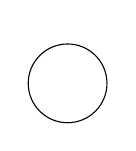
\begin{tikzpicture}
      \draw[white] (0,0) -- (0,0.7); % Just for spacing the table
      \draw (0,0) circle [radius=0.5];
    \end{tikzpicture} &
    \texttt{\bs draw (0,0) circle [radius=0.5];} \\
    \hline
    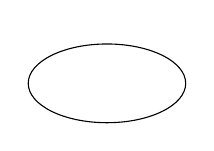
\begin{tikzpicture}
      \draw[white] (0,0) -- (0,0.7); % Just for spacing the table
      \draw (0,0) circle [x radius=1,y radius=0.5];
    \end{tikzpicture} &
    \texttt{\dots [x radius=1,y radius=0.5];} \\
  \end{tabular}
\end{frame}

\begin{frame}[fragile]{Bezier curves}
  \texttt{\bs draw (P1) ..controls (C1) and (C2).. (P2);}

  \vspace{0.5cm}
  \begin{columns}
  \column{0.6\textwidth}
    A curve  from \texttt{P1} to \texttt{P2}, starting in direction of
    \texttt{C1} and arriving from the direction of \texttt{C2} (usually not
    touching the control points).

    \vspace{0.5cm}
    \href{https://en.wikipedia.org/wiki/B\%C3\%A9zier\_curve}
         {https://en.wikipedia.org/wiki/Bézier\_curve}
  \column{0.4\textwidth}
    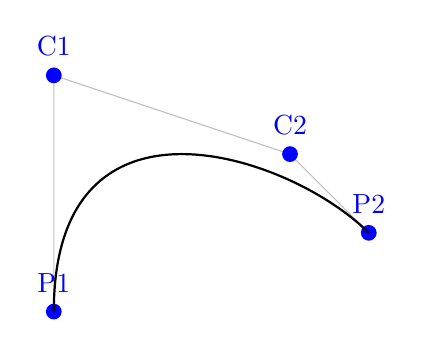
\begin{tikzpicture}
    	\coordinate (P1) at (0,0);
    	\coordinate (P2) at (4,1);
    	\coordinate (C1) at (0,3);
    	\coordinate (C2) at (3,2);
	
    	\draw[lightgray] (P1) foreach \p in {P1,C1,C2,P2} {-- (\p)};
    	\foreach \p in {P1,C1,C2,P2} {
    		\fill[blue] (\p) circle[radius=0.1] node[label=\p] {};
    	};
    	\draw[thick] (P1) ..controls (C1) and (C2).. (P2);
    \end{tikzpicture}
  \end{columns}
\end{frame}

\begin{frame}{Colors}
  \begin{itemize}
    \item Color names already defined: \texttt{red, green, blue, yellow,}
          \texttt{black, white, gray, darkgray, lightgray, brown, pink\dots}

    \vspace{0.2cm}
    \item Specify intensity: \texttt{color!n} with $0\leq n \leq 100$.

    \vspace{0.2cm}
    \item Mix colors: \texttt{color1!n1!color2!n2!\dots}

    \vspace{0.2cm}
    \item Example:
          \begin{center}
            \texttt{blue!50!red!50!green}
          \end{center}
          is 50\% blue, 25\% red and 25\% green.
  \end{itemize}
\end{frame}

\begin{frame}{Filldraw, change color and line style}
  \begin{itemize}
    \item \texttt{\bs draw[\emph{colorname}]} to specify color.

    \vspace{0.2cm}
    \item \texttt{\bs filldraw[fill=\emph{fillcolor}, draw=\emph{bordercolor}]}
          to fill path or \texttt{\bs fill} for no border.

    \vspace{0.2cm}
    \item Line width: \texttt{\bs draw[\emph{thickness}]}, where
          \texttt{\emph{thickness}} can be \texttt{very thin, thin, thick, very
          thick\dots} or \texttt{\bs draw[line width=\emph{length}]} where
          \texttt{\emph{length}} can be \texttt{3pt, 0.1mm\dots}

    \vspace{0.2cm}
    \item Line style: \texttt{[dashed]} for dashed,
          \texttt{[->]} or \texttt{[<-]} for arrow.
  \end{itemize}
\end{frame}


\begin{frame}{Example}
  \begin{center}
    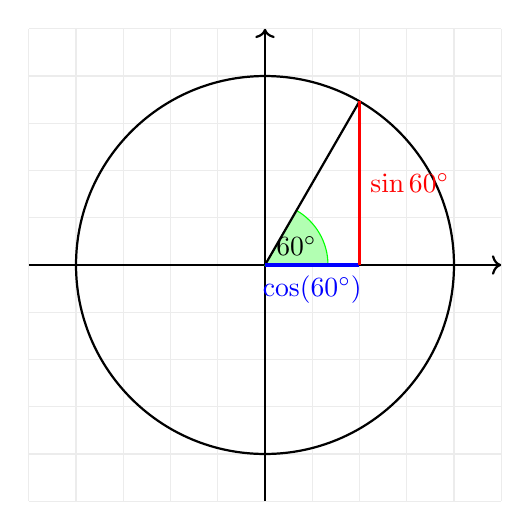
\begin{tikzpicture}[scale=0.6]
    	\colorlet{coscolor}{blue}
    	\colorlet{sincolor}{red}
    	\tikzset{anglefill/.style={draw=green,fill=green!30}}
    	
    	\pgfmathsetmacro{\r}{4}
    	\pgfmathsetmacro{\a}{60}

    	\draw[lightgray!30] (-5,-5) grid[step=1] (5,5);
    	\draw[thick,->] (0,-5) -- (0,5);
    	\draw[thick,->] (-5,0) -- (5,0);
	
    	\filldraw[anglefill] (0,0) -- node[above]{$\a^\circ$}
    	  (\r/3,0) arc [start angle=0,end angle=\a,radius=\r/3] -- cycle;
    	\draw[thick] (0,0) circle[radius=\r] -- (\a:\r);
    	\draw[very thick,coscolor] (0,0) --
    	  node[below]{$\cos(\a^\circ)$} (\r*cos{\a},0);	
    	\draw[very thick,sincolor] (\r*cos{\a},0) --
    	  node[right]{$\sin\a^\circ$}(\a:\r);
    \end{tikzpicture}
  \end{center}
\end{frame}

\begin{frame}{Adding text: nodes}
  \texttt{\bs draw (P1) {\color{red}--} node[\emph{position}]
          \{\emph{text}\} (P2) \dots}

  \vspace{0.5cm}
  \texttt{\bs draw {\color{red}(P1)} node[\emph{position}]
          \{\emph{text}\} -- (P2) \dots}

  \vspace{0.5cm}
  \begin{itemize}
    \item A node can refer to a line or to a point
    \item \texttt{\emph{position}} can be \texttt{above, below, left} or
          \texttt{right}
    \item \texttt{\emph{text}} can also be \texttt{\$math\$}
  \end{itemize}
\end{frame}

\begin{frame}{Macros}
  \texttt{\bs pgfmathsetmacro\{\bs x\}\{\emph{value}\}}

  %\texttt{\bs colorlet\{\emph{colorname}\}\{\emph{color}\}}

  \vspace{0.5cm}
  Examples:

  \vspace{0.2cm}
  \texttt{\bs pgfmathsetmacro\{\bs r\}\{4\}}

  \texttt{\bs pgfmathsetmacro\{\bs a\}\{30\}}
\end{frame}

\begin{frame}[fragile,shrink]{Example - {\ti } code} 
  \begin{verbatim}
  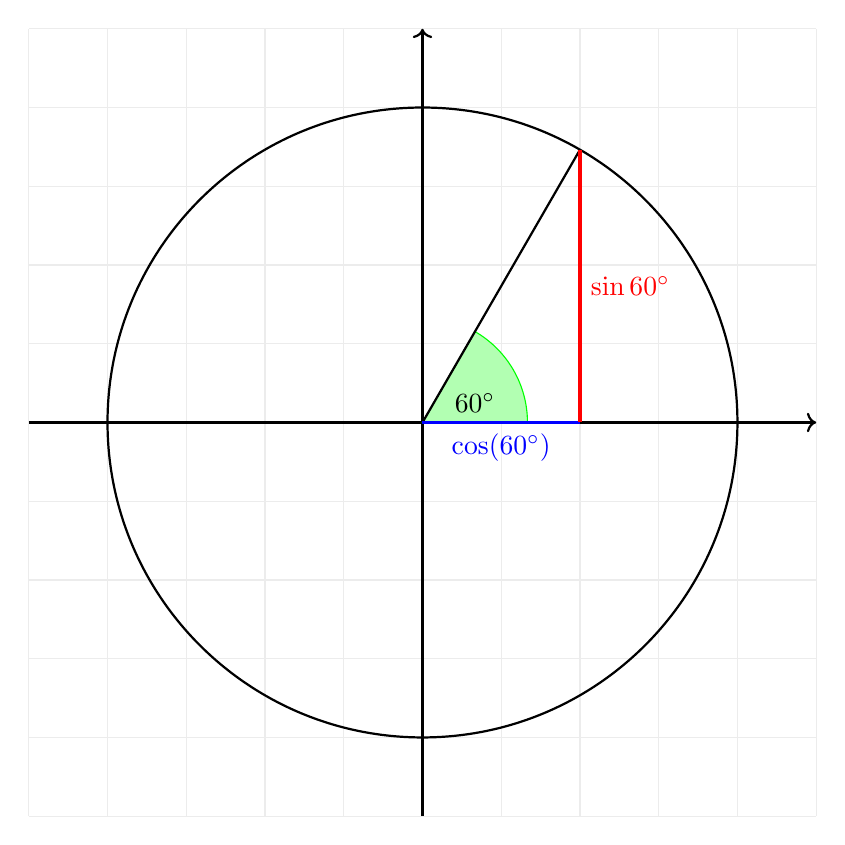
\begin{tikzpicture}
      \colorlet{coscolor}{blue}
      \colorlet{sincolor}{red}
      \tikzset{anglefill/.style={draw=green,fill=green!30}}
      \pgfmathsetmacro{\r}{4}
      \pgfmathsetmacro{\a}{60}

      \draw[lightgray!30] (-5,-5) grid[step=1] (5,5);
      \draw[thick,->] (0,-5) -- (0,5);
      \draw[thick,->] (-5,0) -- (5,0);
	
      \filldraw[anglefill] (0,0) -- node[above]{$\a^\circ$}
          (\r/3,0) arc [start angle=0,end angle=\a,radius=\r/3] -- cycle;
      \draw[thick] (0,0) circle[radius=\r] -- (\a:\r);
      \draw[very thick,coscolor] (0,0) --
          node[below]{$\cos(\a^\circ)$} (\r*cos{\a},0);	
      \draw[very thick,sincolor] (\r*cos{\a},0) --
          node[right]{$\sin\a^\circ$}(\a:\r);
  \end{tikzpicture}
  \end{verbatim}
\end{frame}

\begin{frame}{The \texttt{\bs foreach} command}
  \texttt{\bs foreach \bs i in \{\emph{list}\} \{ \emph{commands} \};}

  \vspace{0.5cm}
  \begin{itemize}
    \item \texttt{\emph{list}} can be fully explicit (like
          \texttt{\{1,7.2,-42\}}) or partially implicit
          (like \texttt{\{1.5,1.6,\dots,5.0\}})
    \item \texttt{\emph{commands}} will be repeated with \texttt{\bs i}
          varying in \texttt{\emph{list}}
    \item One can use \texttt{foreach} inside a \texttt{\bs draw}
  \end{itemize}
\end{frame}

\begin{frame}{\texttt{\bs foreach} examples}
  \begin{tabular}{c|l}
    \tikz \foreach \i in {1,2,3,4} {\draw (\i,0) circle [radius=0.4];}; &
      \begin{tabular}{l}
        \texttt{\bs foreach \bs i in \{1,2,3,4\}} \\
        \texttt{\{\bs draw (\bs i,0) circle [radius=0.4];\}}
      \end{tabular} \\
    \tikz[scale=2]\draw (0,0) \foreach\i in {0.0,0.3,...,1.5} {-- (\i,\i^2)}; &
      \begin{tabular}{l}
        \texttt{\bs draw (0,0) \bs foreach \bs i in} \\
        \texttt{  \{0.0,0.3,...,1.5\} \{-- (\bs i,\bs i\^{}2)\};}
      \end{tabular}
  \end{tabular}
\end{frame}

\begin{frame}{External packages}
  Many external packages, include with \texttt{\bs usepackage}:
  \url{https://www.ctan.org/topic/pgf-tikz}

  \vspace{0.3cm}
  \begin{itemize}
    \item Graphs and similar: \texttt{tikz-cd, adigraph, binarytree\dots}
    \item Diagrams: \texttt{pgf-pie, bchart, venndiagram\dots}
    \item Other sciences: \texttt{chemfig, CircuiTikZ\dots}
    \item Fun: \texttt{battleship, TikZducks, tikz-among-us\dots}
  \end{itemize}
\end{frame}

\begin{frame}[fragile]{Commutative diagrams}
  \begin{center}
    \begin{tikzcd}
      T \arrow[drr, bend left, "x"] \arrow[ddr, bend right, "y"']
        \arrow[dr, dotted, "{(x,y)}" description] & & \\
      & X \times_Z Y \arrow[r, "p"] \arrow[d, "q"] & X \arrow[d, "f"] \\
      & Y \arrow[r, "g"] & Z
    \end{tikzcd}
  \end{center}
\end{frame}

\begin{frame}{tikz-cd}

  Reference:
  {\footnotesize
  \url{http://ctan.cs.uu.nl/graphics/pgf/contrib/tikz-cd/tikz-cd-doc.pdf}}

  \vspace{0.7cm}
  \texttt{\bs usepackage\{tikz-cd\}}

  \vspace{0.2cm}
  \texttt{\bs begin\{tikzcd\}\dots \bs end\{tikzcd\}}

  \vspace{0.5cm}
  \begin{itemize}
    \item Works as a \texttt{tabular} or \texttt{matrix} (with \texttt{\&} and
          \texttt{\bs\bs})
    \item Everything is in math mode by default
  \end{itemize}
\end{frame}

\begin{frame}{Arrows}
  \texttt{\bs arrow[\emph{direction},"label",other options]}

  \vspace{0.5cm}
  \begin{itemize}
    \item \texttt{\emph{direction}} can be any combination of the letters
          \texttt r (right), \texttt l (left), \texttt d (down) and
          \texttt u (up)
    \item The target must exist:
          \begin{center}
            \begin{tabular}{ll}
              \texttt{X \bs arrow[r] \& Y} & \texttt{\% Ok} \\
              \texttt{X \bs arrow[r] } & \texttt{\% Error}  \\
              \texttt{X \bs arrow[r] \& \{\}} & \texttt{\% Ok}
            \end{tabular}
          \end{center}
    \item Other options describe the shape and style of the arrow

  \end{itemize}
\end{frame}

\begin{frame}[fragile]{Examples}
  \begin{tabular}{c|l}
    \begin{tikzcd} X\arrow[r,dashed,"f"] & Y \end{tikzcd} &
      \begin{tabular}{l}
        \texttt{X \bs arrow[r,dashed,"f"] \& Y}
      \end{tabular} \\
    & \quad \\
    \begin{tikzcd}
      A\arrow[r,bend right,"\pi^2"] & B\arrow[r,bend left,tail] & C
    \end{tikzcd} &
      \begin{tabular}{l}
        \texttt{A \bs arrow[r,bend right,"\bs pi\^{}2"] \&} \\
        \texttt{B \bs arrow[r,bend left,tail] \& C}
      \end{tabular} \\
    & \quad \\
    \begin{tikzcd}
      A \arrow[d,"1"'] \arrow[dr,"2"] & B \\
      C & D \arrow[l] \arrow[u,out=45,in=0]
    \end{tikzcd} &
      \begin{tabular}{l}
        \texttt{A \bs arrow[d,"1"'] \bs arrow[dr,"2"] \& B \bs\bs} \\
        \texttt{C \& D \bs arrow[l] \bs arrow[u,out=45,in=0]}
      \end{tabular}
  \end{tabular}
\end{frame}

\end{document}

